%%%%%%%%%%%%%%%%%%%%%%%%%%%%%%%%%%%%%%
%%%%%%%%%%%%%%%%%%%%%%%%%%%%%%%%%%%%%%
% Do not edit the TeX file your work
% will be overwritten.  Edit the RnW
% file instead.
%%%%%%%%%%%%%%%%%%%%%%%%%%%%%%%%%%%%%%
%%%%%%%%%%%%%%%%%%%%%%%%%%%%%%%%%%%%%%




On the Iris data, we evaluated the expected number of clusters for a range of
$\alpha$ between 0.5 and 6.5. Then we chose three $\alpha_0$ values, 2, 3.5, and
5, and constructed the linear approximation centered at each of these
$\alpha_0$s. The linear approximation did quite well for choices of $\alpha$
close to $\alpha_0$, as seen in \prettyref{fig:parametric_sens_plot}.
%  Hence, by evaluating the objective at three $\alpha_0$s, we
% can use the linear approximation to understand the effect of the DP prior
% parameter $\alpha$ across the entire range from 0.5 - 6.5.


\begin{knitrout}
\definecolor{shadecolor}{rgb}{0.969, 0.969, 0.969}\color{fgcolor}\begin{figure}[!h]

{\centering 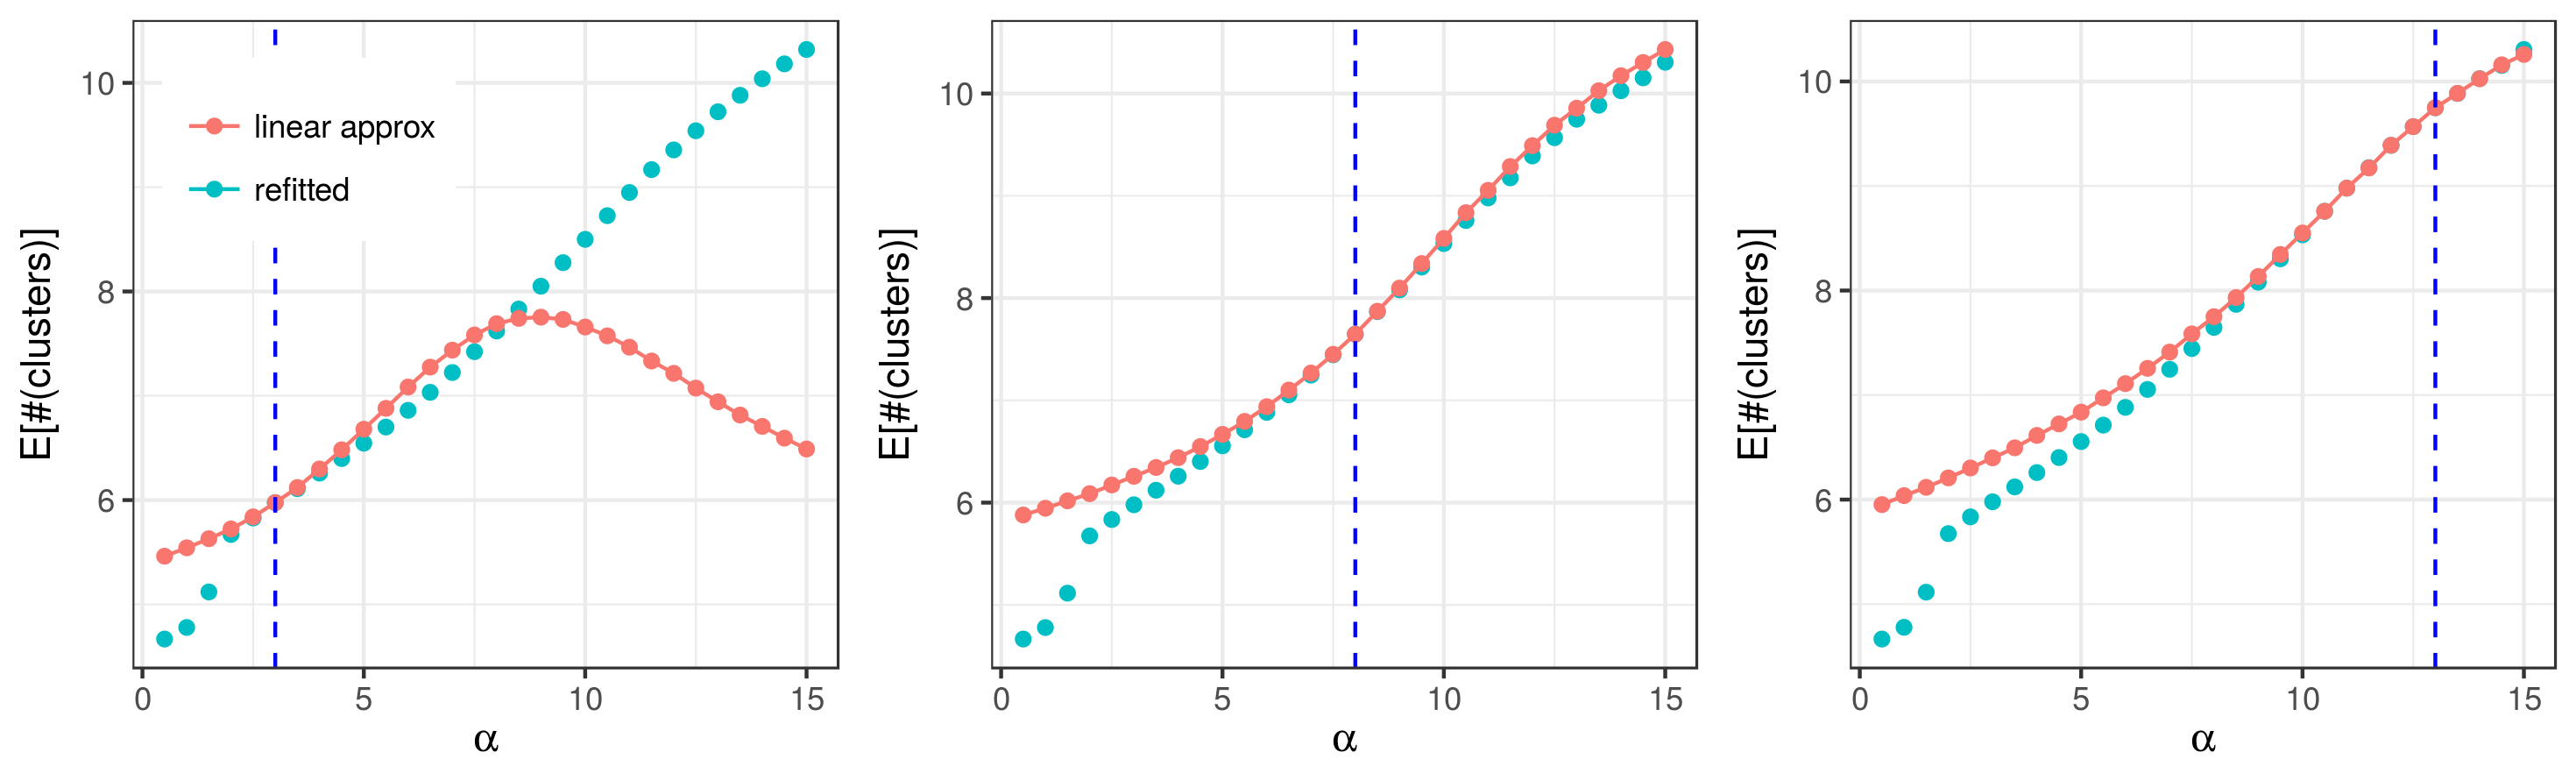
\includegraphics[width=0.98\linewidth,height=0.294\linewidth]{figure/parametric_sens_plot-1} 

}

\caption[Comparison of the expected number of clusters computed by re-optimizing versus the linear approximation]{Comparison of the expected number of clusters computed by re-optimizing versus the linear approximation.  The blue vertical line indicates the location of $\alpha_0$.}\label{fig:parametric_sens_plot}
\end{figure}


\end{knitrout}
